\chapter{Quadro Terminal para Painel Led 9x3}
Este capítulo mostra os valores efetivos para a confecção do quadro para o Painel LED Full Color. Foram usados os métodos de dimensionamento explicados no Capítulo \ref{cap:calculos}. Nas próximas seções, serão apresentados os parâmetros de projeto utilizados, a tabela de carga, os diagramas unifilar e multifilar e uma representação gráfica do quadro (esquema funcional) nas opções simples. Ao final, há uma lista de materiais para montagem.

\section{Parâmetros de projeto}

O Painel Full Color Led 9x3 é composto por 27 gabinetes e deve ser alimentado com 9 cabos de força. Há três opções de resolução (P10, P8 e P5), cada uma com sua potência. A Tabela \ref{tab:pot_9x3} apresenta as informações de potência de cada gabinete, a quantidade de cabos ou grupos de até 3 gabinetes para conectar à rede elétrica e a quantidade de gabinetes e a potência total do Painel.

\begin{table}[htbp]
\caption{Potência Painel LED 9x3}
\centering
\begin{tabular}{cccccc}
\toprule
\multirow{2}{*}{Item} & \multirow{2}{*}{Tipo} & \multirow{2}{*}{Potência (W)} & \multicolumn{3}{c}{Painéis} \\
\cmidrule{4-6}
& & & Cabos  & Gabinete & Potência Total (W) \\
\midrule


34 & P8 & 630 & 9 & 27 & 17010 \\
35 & P5 & 684 & 9 & 27 & 18468 \\
36 & P10 & 540 & 9 & 27 & 14580 \\


\bottomrule
\end{tabular}
\label{tab:pot_9x3}
\end{table}


\section{Tabela de Carga}



\begin{landscape}
\begin{center}
\large\textbf{Tabela Grande}
\end{center}
\begin{tabular}{|c|c|c|c|}
%conteúdo da tabela grande
\end{tabular}
\vfill % preenche espaço vertical com espaço em branco

\begin{minipage}[t]{0.49\linewidth} % primeira coluna da parte de baixo
\centering
\large\textbf{Tabela Menor}
\begin{tabular}{|c|c|c|}
%conteúdo da tabela menor
\end{tabular}
\end{minipage}
\hfill % preenche espaço horizontal entre as colunas com espaço em branco
\begin{minipage}[t]{0.49\linewidth} % segunda coluna da parte de baixo
\centering
\large\textbf{Observações}
%conteúdo das observações
\end{minipage}

\end{landscape}

\subsection{Trifásico 127/220 V}

\begin{table}[htbp]
\centering
\caption{Tabela de Carga QT para painel Led 9x3 P10 trifásico 127/ 220V}
\resizebox{\linewidth}{!}{
\begin{tabular}{@{}llccccccccc@{}}
\toprule
Circ. & Descr. & Gab. & Polos & Potência & dist L (m) & Ib & Cabo  & DTM & DTM &  \\ 
 		&  		& P5 (Qtd) & tipo&  (W) & (m) 		& (A) & (mm²) & (A) & BCD & \\ 
 		\midrule
1 & Grupo 1 & 3 & Monofásico & 1.620 & 5 & 13 & 3 & 16 & C &  \\ 
2 & Grupo 2 & 3 & Monofásico & 1.620 & 5 & 13 & 3 & 16 & C &  \\
3 & Grupo 3 & 3 & Monofásico & 1.620 & 5 & 13 & 3 & 16 & C & \\ 
4 & Grupo 4 & 3 & Monofásico & 1.620 & 5 & 13 & 3 & 16 & C &  \\ 
5 & Grupo 5 & 3 & Monofásico & 1.620 & 5 & 13 & 3 & 16 & C &  \\ 
6 & Grupo 6 & 3 & Monofásico & 1.620 & 5 & 13 & 3 & 16 & C &  \\ 
7 & Grupo 7 & 3 & Monofásico & 1.620 & 5 & 13 & 3 & 16 & C &  \\ 
8 & Grupo 8 & 3 & Monofásico & 1.620 & 5 & 13 & 3 & 16 & C &  \\ 
9 & Grupo 9 & 3 & Monofásico & 1.620 & 5 & 13 & 3 & 16 & C &  \\ 
10 & Comunicação & 1 & Monofásico & 540 & 0 & 4 & 3 & 10 & C & \\ 
 & Geral &  & Trifásico & 15.120 & 50 & 43 & 16 & 50 & C &  \\
 \bottomrule
\end{tabular}
}
\label{tab:carga9x3T220P10}
\end{table}

\begin{table}[htbp]
\centering
\caption{Tabela de Carga QT para painel Led 9x3 P8 trifásico 127/ 220V}
\resizebox{\linewidth}{!}{
\begin{tabular}{|c|c|c|c|c|c|c|c|c|c|c|c|c|}
\hline
Circuito & Descrição & Gabinetes & Circuito & Potência & dist L (m) & \multicolumn{1}{l|}{Corrente proj} & Cabo  & DTM & DTM & FASES &  &  \\ \hline
 &  & P8 (Qtd) &  &  (W) & (m) & Ib (A) & (mm²) & (A) & Clase & \multicolumn{ 3}{c|}{R} \\ \cline{ 1- 10}
1 & Grupo 1 & 3 & Monofásico & 1.890 & 5 & 15 & 3 & 20 & C & 1.890 & 0 & 0 \\ \hline
2 & Grupo 2 & 3 & Monofásico & 1.890 & 5 & 15 & 3 & 20 & C & 0 & 1.890 & 0 \\ \hline
3 & Grupo 3 & 3 & Monofásico & 1.890 & 5 & 15 & 3 & 20 & C & 0 & 0 & 1.890 \\ \hline
4 & Grupo 4 & 3 & Monofásico & 1.890 & 5 & 15 & 3 & 20 & C & 1.890 & 0 & 0 \\ \hline
5 & Grupo 5 & 3 & Monofásico & 1.890 & 5 & 15 & 3 & 20 & C & 0 & 1.890 & 0 \\ \hline
6 & Grupo 6 & 3 & Monofásico & 1.890 & 5 & 15 & 3 & 20 & C & 0 & 0 & 1.890 \\ \hline
7 & Grupo 7 & 3 & Monofásico & 1.890 & 5 & 15 & 3 & 20 & C & 1.890 & 0 & 0 \\ \hline
8 & Grupo 8 & 3 & Monofásico & 1.890 & 5 & 15 & 3 & 20 & C & 0 & 1.890 & 0 \\ \hline
9 & Grupo 9 & 3 & Monofásico & 1.890 & 5 & 15 & 3 & 20 & C & 0 & 0 & 1.890 \\ \hline
10 & Comunicação & 1 & Monofásico & 630 & 0 & 5 & 3 & 16 & C & 630 & 0 & 0 \\ \hline
 & Geral &  & Trifásico & 17.640 & 80 & 50 & 16 & 50 & C & 6.300 & 5.670 & 5.670 \\ \hline
\end{tabular}
}
\label{tab:carga9x3T220P8}
\end{table}

\begin{table}[htbp]
\centering
\caption{Tabela de Carga QT para painel Led 9x3 P5 trifásico 127/ 220V}
\resizebox{\linewidth}{!}{
\begin{tabular}{|c|l|r|l|r|r|r|r|r|l|l|l|l|}
\hline
Circuito & \multicolumn{1}{c|}{Descrição} & \multicolumn{1}{c|}{Gabinetes} & \multicolumn{1}{c|}{Circuito} & \multicolumn{1}{c|}{Potência} & \multicolumn{1}{c|}{dist L (m)} & \multicolumn{1}{l|}{Corrente proj} & \multicolumn{1}{c|}{Cabo } & \multicolumn{1}{c|}{DTM} & \multicolumn{1}{c|}{DTM} & \multicolumn{1}{c|}{FASES} & \multicolumn{1}{c|}{} & \multicolumn{1}{c|}{} \\ \hline
 & \multicolumn{1}{c|}{} & \multicolumn{1}{c|}{P5 (Qtd)} & \multicolumn{1}{c|}{} & \multicolumn{1}{c|}{ (W)} & \multicolumn{1}{c|}{(m)} & \multicolumn{1}{c|}{Ib (A)} & \multicolumn{1}{c|}{(mm²)} & \multicolumn{1}{c|}{(A)} & \multicolumn{1}{c|}{Clase} & \multicolumn{ 3}{c|}{R} \\ \cline{ 1- 10}
1 & Grupo 1 & 3 & Monofásico & 2.052 & 5 & 16 & 3 & 20 & C & \multicolumn{1}{r|}{2.052} & 0 & 0 \\ \hline
2 & Grupo 2 & 3 & Monofásico & 2.052 & 5 & 16 & 3 & 20 & C & 0 & \multicolumn{1}{r|}{2.052} & 0 \\ \hline
3 & Grupo 3 & 3 & Monofásico & 2.052 & 5 & 16 & 3 & 20 & C & 0 & 0 & \multicolumn{1}{r|}{2.052} \\ \hline
4 & Grupo 4 & 3 & Monofásico & 2.052 & 5 & 16 & 3 & 20 & C & \multicolumn{1}{r|}{2.052} & 0 & 0 \\ \hline
5 & Grupo 5 & 3 & Monofásico & 2.052 & 5 & 16 & 3 & 20 & C & 0 & \multicolumn{1}{r|}{2.052} & 0 \\ \hline
6 & Grupo 6 & 3 & Monofásico & 2.052 & 5 & 16 & 3 & 20 & C & 0 & 0 & \multicolumn{1}{r|}{2.052} \\ \hline
7 & Grupo 7 & 3 & Monofásico & 2.052 & 5 & 16 & 3 & 20 & C & \multicolumn{1}{r|}{2.052} & 0 & 0 \\ \hline
8 & Grupo 8 & 3 & Monofásico & 2.052 & 5 & 16 & 3 & 20 & C & 0 & \multicolumn{1}{r|}{2.052} & 0 \\ \hline
9 & Grupo 9 & 3 & Monofásico & 2.052 & 5 & 16 & 3 & 20 & C & 0 & 0 & \multicolumn{1}{r|}{2.052} \\ \hline
10 & Comunicação & 1 & Monofásico & 684 & 0 & 5 & 3 & 16 & C & \multicolumn{1}{r|}{684} & 0 & 0 \\ \hline
 & Geral & \multicolumn{1}{l|}{} & Trifásico & 19.152 & 100 & 55 & 25 & 63 & C & \multicolumn{1}{r|}{6.840} & \multicolumn{1}{r|}{6.156} & \multicolumn{1}{r|}{6.156} \\ \hline
\end{tabular}
}
\label{tab:carga9x3T220P5}
\end{table}



\subsection{Trifásico 220/380 V}
\begin{table}[htbp]
\centering
\caption{Tabela de Carga QT para painel Led 9x3 P10 trifásico  220/380V}

\resizebox{\linewidth}{!}{
\begin{tabular}{|c|c|c|c|c|c|c|c|c|c|c|c|c|}
\hline
Circuito & Descrição & Gabinetes & Circuito & Potência & dist L (m) & \multicolumn{1}{l|}{Corrente proj} & Cabo  & DTM & DTM & \multicolumn{ 3}{c|}{FASES} \\ \hline
 &  & P10 (Qtd) &  &  (W) & (m) & Ib (A) & (mm²) & (A) & Clase & R & S & T \\ \hline
1 & Grupo 1 & 3 & Monofásico & 1.620 & 5 & 7 & 3 & 16 & C & 1.620 & 0 & 0 \\ \hline
2 & Grupo 2 & 3 & Monofásico & 1.620 & 5 & 7 & 3 & 16 & C & 0 & 1.620 & 0 \\ \hline
3 & Grupo 3 & 3 & Monofásico & 1.620 & 5 & 7 & 3 & 16 & C & 0 & 0 & 1.620 \\ \hline
4 & Grupo 4 & 3 & Monofásico & 1.620 & 5 & 7 & 3 & 16 & C & 1.620 & 0 & 0 \\ \hline
5 & Grupo 5 & 3 & Monofásico & 1.620 & 5 & 7 & 3 & 16 & C & 0 & 1.620 & 0 \\ \hline
6 & Grupo 6 & 3 & Monofásico & 1.620 & 5 & 7 & 3 & 16 & C & 0 & 0 & 1.620 \\ \hline
7 & Grupo 7 & 3 & Monofásico & 1.620 & 5 & 7 & 3 & 16 & C & 1.620 & 0 & 0 \\ \hline
8 & Grupo 8 & 3 & Monofásico & 1.620 & 5 & 7 & 3 & 16 & C & 0 & 1.620 & 0 \\ \hline
9 & Grupo 9 & 3 & Monofásico & 1.620 & 5 & 7 & 3 & 16 & C & 0 & 0 & 1.620 \\ \hline
10 & Comunicação & 1 & Monofásico & 540 & 0 & 2 & 3 & 16 & C & 540 & 0 & 0 \\ \hline
 & Geral &  & Trifásico & 15.120 & 90 & 25 & 6 & 32 & C & 5.400 & 4.860 & 4.860 \\ \hline
\end{tabular}
}
\label{tab:carga9x3T380P10}
\end{table}

\begin{table}[htbp]
\centering
\caption{Tabela de Carga QT para painel Led 9x3 P8 trifásico  220/380V}

\resizebox{\linewidth}{!}{
\begin{tabular}{|c|c|c|c|c|c|c|c|c|c|c|c|c|}
\hline
Circuito & Descrição & Gabinetes & Circuito & Potência & dist L (m) & \multicolumn{1}{l|}{Corrente proj} & Cabo  & DTM & DTM & FASES &  &  \\ \hline
 &  & P8 (Qtd) &  &  (W) & (m) & Ib (A) & (mm²) & (A) & Clase & \multicolumn{ 3}{c|}{R} \\ \cline{ 1- 10}
1 & Grupo 1 & 3 & Monofásico & 1.890 & 5 & 9 & 3 & 16 & C & 1.890 & 0 & 0 \\ \hline
2 & Grupo 2 & 3 & Monofásico & 1.890 & 5 & 9 & 3 & 16 & C & 0 & 1.890 & 0 \\ \hline
3 & Grupo 3 & 3 & Monofásico & 1.890 & 5 & 9 & 3 & 16 & C & 0 & 0 & 1.890 \\ \hline
4 & Grupo 4 & 3 & Monofásico & 1.890 & 5 & 9 & 3 & 16 & C & 1.890 & 0 & 0 \\ \hline
5 & Grupo 5 & 3 & Monofásico & 1.890 & 5 & 9 & 3 & 16 & C & 0 & 1.890 & 0 \\ \hline
6 & Grupo 6 & 3 & Monofásico & 1.890 & 5 & 9 & 3 & 16 & C & 0 & 0 & 1.890 \\ \hline
7 & Grupo 7 & 3 & Monofásico & 1.890 & 5 & 9 & 3 & 16 & C & 1.890 & 0 & 0 \\ \hline
8 & Grupo 8 & 3 & Monofásico & 1.890 & 5 & 9 & 3 & 16 & C & 0 & 1.890 & 0 \\ \hline
9 & Grupo 9 & 3 & Monofásico & 1.890 & 5 & 9 & 3 & 16 & C & 0 & 0 & 1.890 \\ \hline
10 & Comunicação & 1 & Monofásico & 630 & 0 & 3 & 3 & 10 & C & 630 & 0 & 0 \\ \hline
 & Geral &  & Trifásico & 17.640 & 70 & 29 & 6 & 32 & C & 6.300 & 5.670 & 5.670 \\ \hline
\end{tabular}
}
\label{tab:carga9x3T380P8}
\end{table}

\begin{landscape}
\begin{table}[htbp]
\centering
\caption{Tabela de Carga QT para painel Led 9x3 P5 trifásico  220/380V}
\begin{tabular}{|c|c|c|c|c|c|c|c|c|c|c|c|c|}
\hline
Circuito & Descrição & Gabinetes & Circuito & Potência & dist L (m) & \multicolumn{1}{l|}{Corrente proj} & Cabo  & DTM & DTM & FASES &  &  \\ \hline
 &  & P5 (Qtd) &  &  (W) & (m) & Ib (A) & (mm²) & (A) & Clase & \multicolumn{ 3}{c|}{R} \\ \cline{ 1- 10}
1 & Grupo 1 & 3 & Monofásico & 2.052 & 5 & 9 & 3 & 16 & C & 2.052 & 0 & 0 \\ \hline
2 & Grupo 2 & 3 & Monofásico & 2.052 & 5 & 9 & 3 & 16 & C & 0 & 2.052 & 0 \\ \hline
3 & Grupo 3 & 3 & Monofásico & 2.052 & 5 & 9 & 3 & 16 & C & 0 & 0 & 2.052 \\ \hline
4 & Grupo 4 & 3 & Monofásico & 2.052 & 5 & 9 & 3 & 16 & C & 2.052 & 0 & 0 \\ \hline
5 & Grupo 5 & 3 & Monofásico & 2.052 & 5 & 9 & 3 & 16 & C & 0 & 2.052 & 0 \\ \hline
6 & Grupo 6 & 3 & Monofásico & 2.052 & 5 & 9 & 3 & 16 & C & 0 & 0 & 2.052 \\ \hline
7 & Grupo 7 & 3 & Monofásico & 2.052 & 5 & 9 & 3 & 16 & C & 2.052 & 0 & 0 \\ \hline
8 & Grupo 8 & 3 & Monofásico & 2.052 & 5 & 9 & 3 & 16 & C & 0 & 2.052 & 0 \\ \hline
9 & Grupo 9 & 3 & Monofásico & 2.052 & 5 & 9 & 3 & 16 & C & 0 & 0 & 2.052 \\ \hline
10 & Comunicação & 1 & Monofásico & 684 & 0 & 3 & 3 & 10 & C & 684 & 0 & 0 \\ \hline
 & Geral &  & Trifásico & 19.152 & 60 & 32 & 10 & 32 & C & 6.840 & 6.156 & 6.156 \\ \hline
\end{tabular}
\label{tab:carga9x3T380P5}
\end{table}
\end{landscape}


\section{Diagrama Unifilar}
Apresentação dos diagramas unifilare completos para o quadro de alimentação dos paineis 9x3
As ligações do quadro são compativeis com o esquema TN-S ou TN-S-C de proteção equipotencial (aterramento). Ou seja, condutores neutro e de aterramento separados. 


\subsection{Trifásico 127/220 V}
Diagrama trifásico 127/220V P5 Figura \ref{fig:unifilar9x3220p5} - Detalhado na folha de projeto 

\begin{figure}[h]
    \centering
    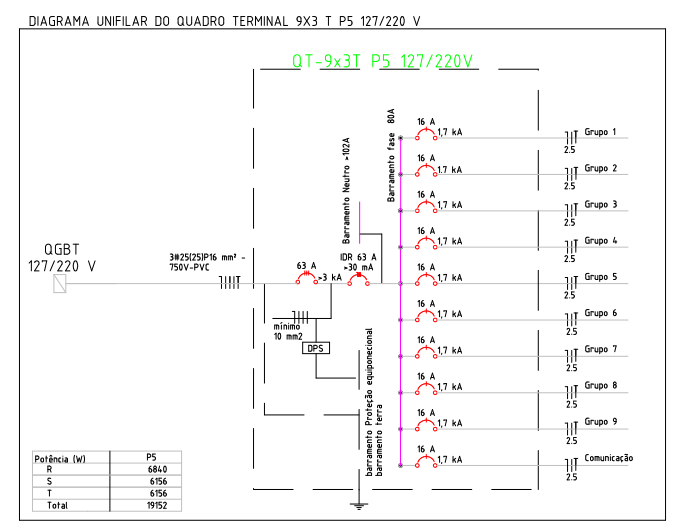
\includegraphics[width=0.6\textwidth]{image/DU9X3T220P5.png}
    %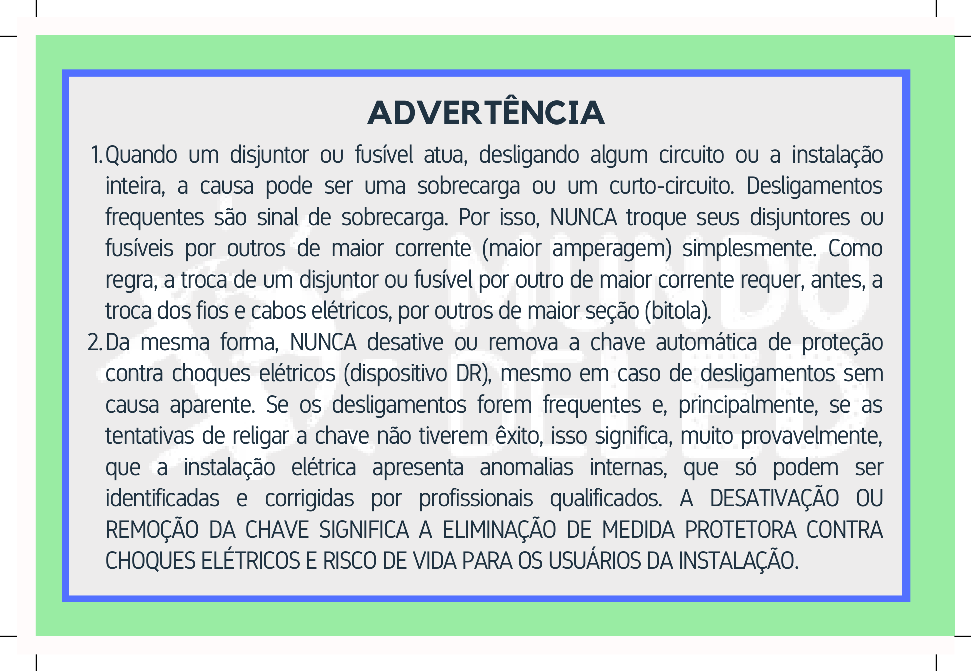
\includegraphics[width=4cm]{image/EtiqAdvQD.pdf}
    \caption{Diagrama unifilar do quadro terminal para painel full color 9x3 P5 trifásico 127/220V}
   \label{fig:unifilar9x3220p5}
\end{figure}
Diagrama trifásico 127/220V P8 e P10 Figura \ref{fig:unifilar9x3220p8p10} - Detalhado na folha de projeto
\begin{figure}[h]
    \centering
    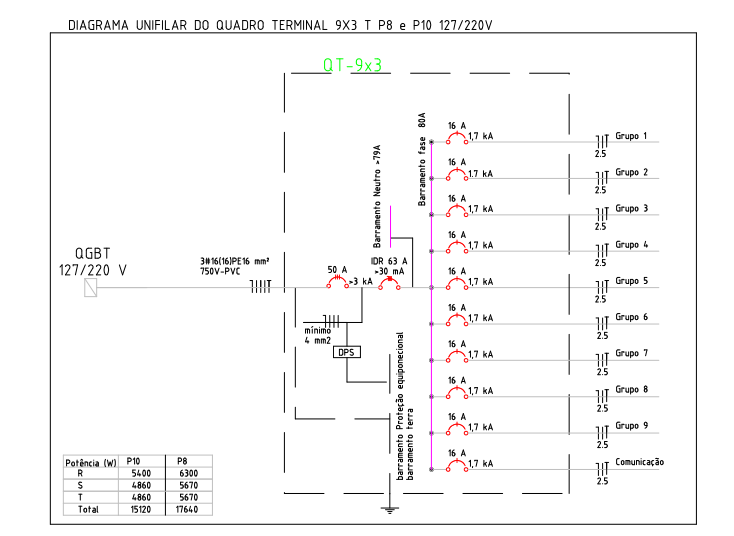
\includegraphics[width=0.6\textwidth]{image/DU9X3T220P8P10.png}
    %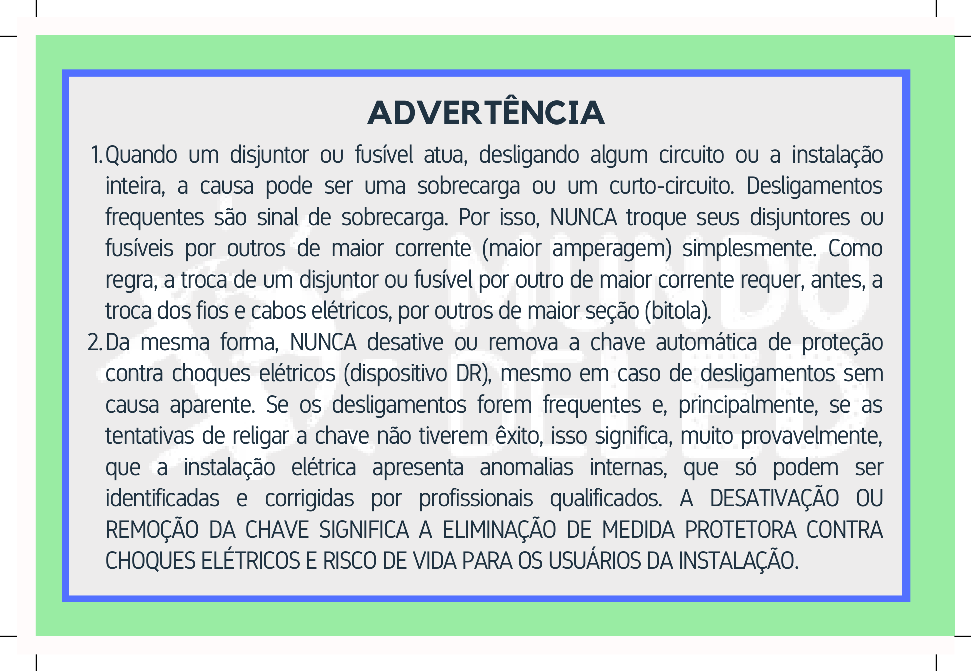
\includegraphics[width=4cm]{image/EtiqAdvQD.pdf}
    \caption{Diagrama unifilar do quadro terminal para painel full color 9x3 P5 trifásico 127/220V}
   \label{fig:unifilar9x3220p8p10}
\end{figure}

\subsection{Trifásico 220/380 V}
Diagrama trifásico 220/380V P5 Figura \ref{fig:unifilar9x3220p5} - Detalhado na folha de projeto
\begin{figure}[h]
    \centering
    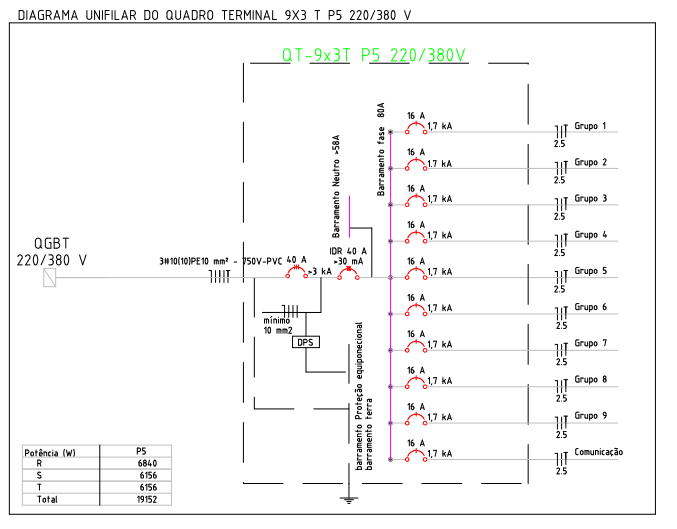
\includegraphics[width=0.6\textwidth]{image/DU9X3T380P5.png}
    %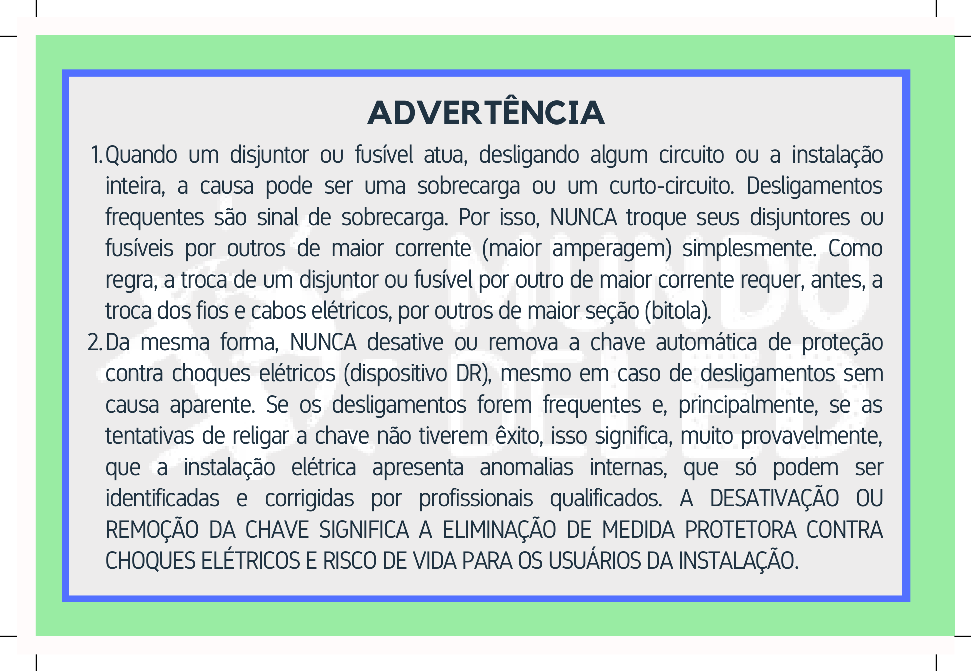
\includegraphics[width=4cm]{image/EtiqAdvQD.pdf}
    \caption{Diagrama unifilar do quadro terminal para painel full color 9x3 P5 trifásico 127/220V}
   \label{fig:unifilar9x33800p5}
\end{figure}
Diagrama trifásico 220/380V P8 e P10 Figura \ref{fig:unifilar9x3220p8p10} - Detalhado na folha de projeto
\begin{figure}[h]
    \centering
    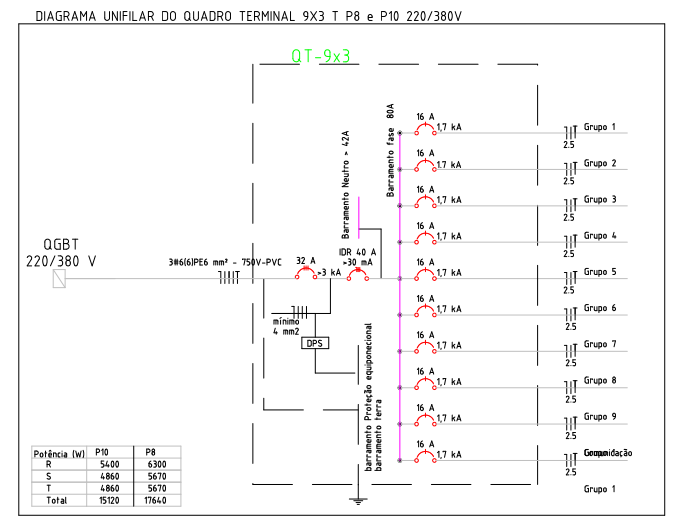
\includegraphics[width=0.6\textwidth]{image/DU9X3T380P8P10.png}
    %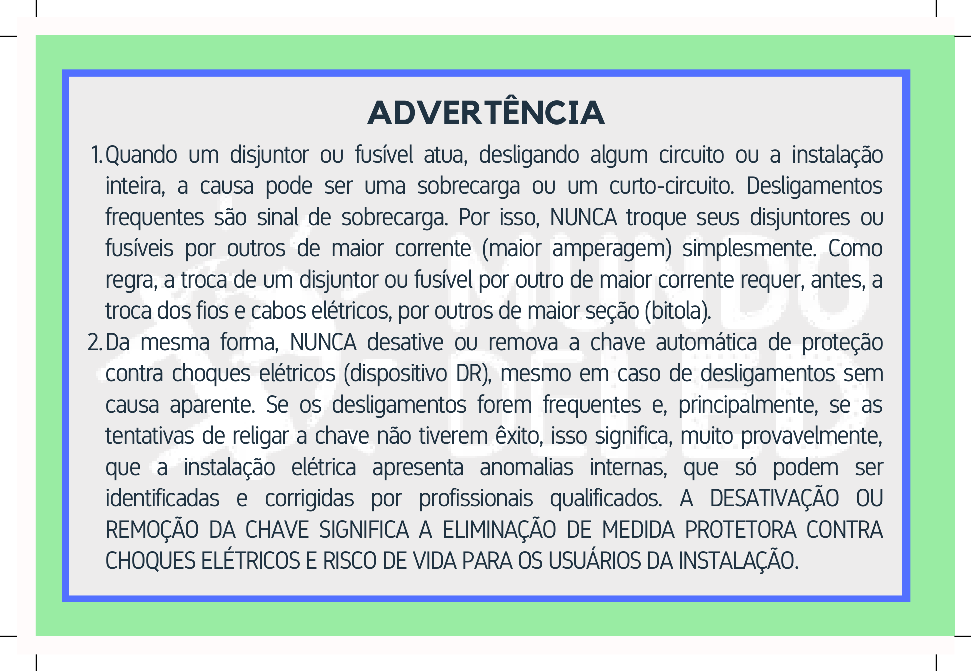
\includegraphics[width=4cm]{image/EtiqAdvQD.pdf}
    \caption{Diagrama unifilar do quadro terminal para painel full color 9x3 P5 trifásico 127/220V}
   \label{fig:unifilar9x33800p8p10}
\end{figure}

\section{Diagrama Multifilar}
Diagrama multifilar representa o esquema de ligação indicando as entradas, saídas e conexões do quadro. A seguir diagramas multifilar para as tensões entre fase 220V e 380V. Cada diagrama tem as infomações para os modulos P5, P8 e P10.
\subsection{Diagrama Multifilar do Quadro Terminal Trifásico 127/220V} 

\begin{figure}[h]
    \centering
    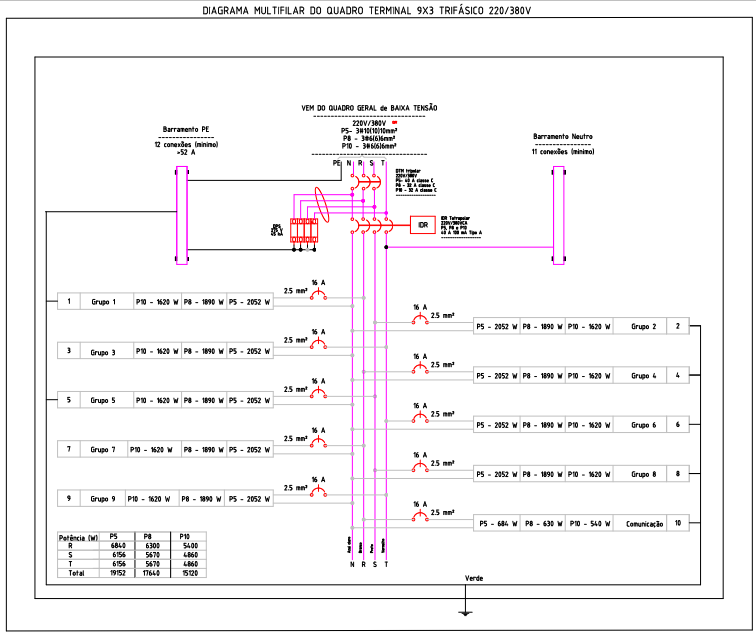
\includegraphics[width=\textwidth]{image/multi9x3t220.png}
    %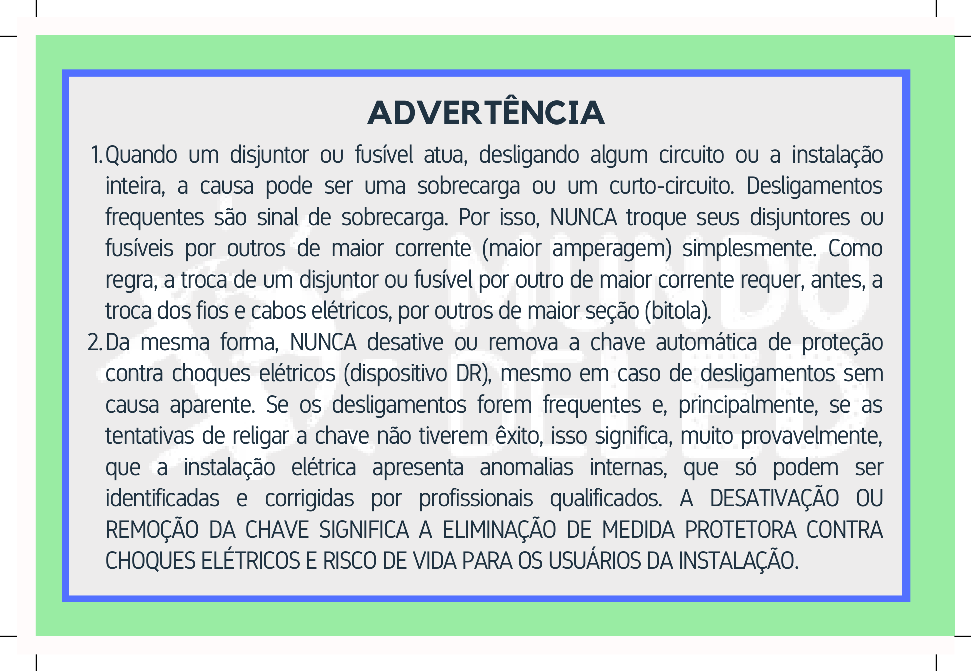
\includegraphics[width=4cm]{image/EtiqAdvQD.pdf}
    \caption{Representação gráfica do layout interno do quadro de energia para o Painel 9x3T completo}
   \label{fig:QDTmult9x3t220}
\end{figure}

\subsection{Diagrama Multifilar do Quadro Terminal Trifásico 220/380V} 

\begin{figure}[h]
    \centering
    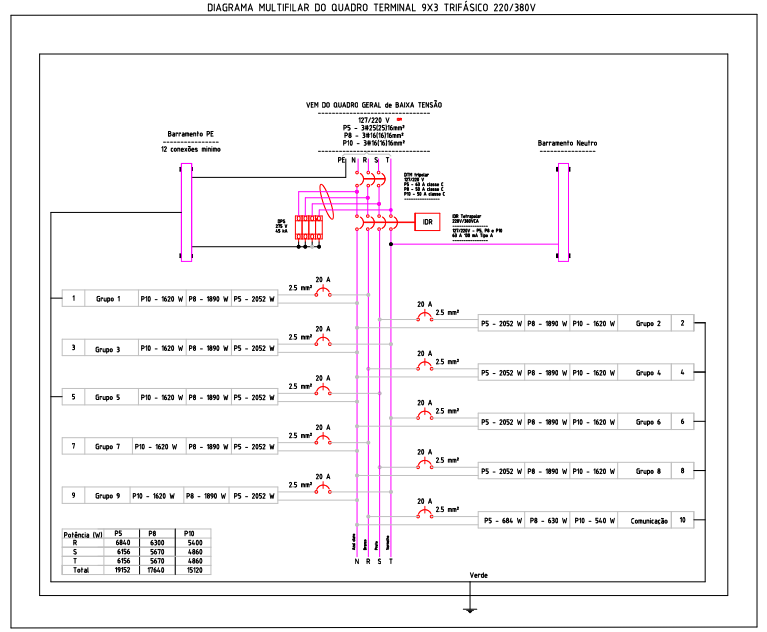
\includegraphics[width=\textwidth]{image/multi9x3t380.png}
    %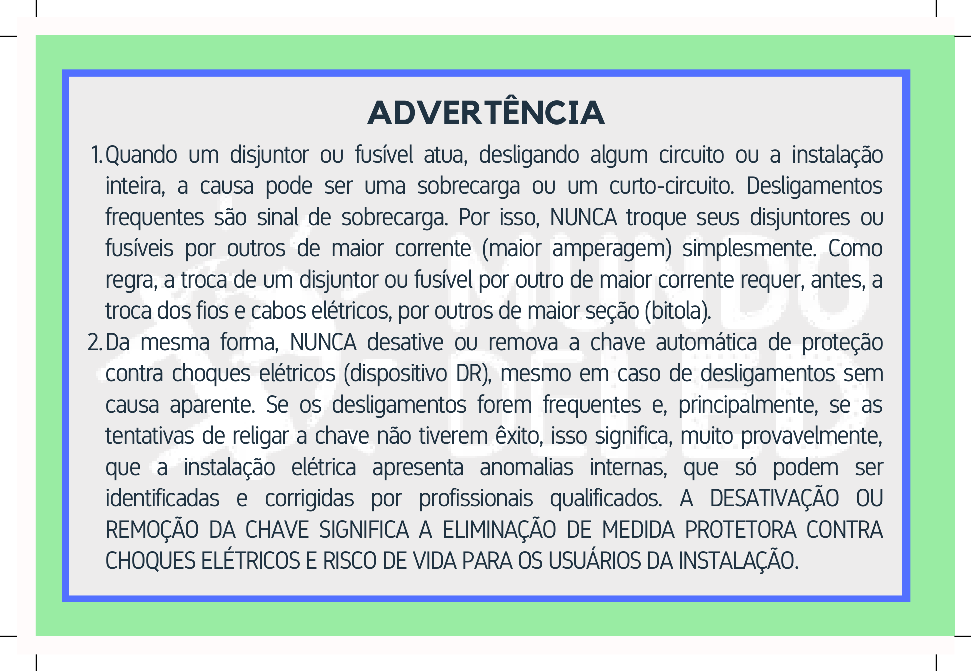
\includegraphics[width=4cm]{image/EtiqAdvQD.pdf}
    \caption{Representação gráfica do layout interno do quadro de energia para o Painel 9x3T completo}
   \label{fig:QDTmult9x3t380}
\end{figure}


%\subsection{Trifásico 127/220 V}

%\subsection{Trifásico 220/380 V}

\section{Representação geral de disposição dos componentes no quadro terminal}
A disposição aqui é uma sugestão de layout. A disposição dos componentes poderá ser alterada conforme conveniêcia, desde o esquema de ligação elétrica do projeto não seja alterado e q ue todas as restrição/recomendações do fabricante do componente sejam atendidas.
Na figura \ref{fig:QDlayout9x3} um layout para quadro completo, indicado principalmente para exposição na área externa. 
O quadro para Painel 9x3m é composto por 10 circuitos terminais, 9 para ligar os grupos de até 3 paineis, através do cabo de força. Um circuito para as tomadas internas que tem a finalidade de alimentar o dispositivo de comunicação e controle do Painel.

Potência máxima de cada circuito terminal


\begin{figure}[h]
    \centering
    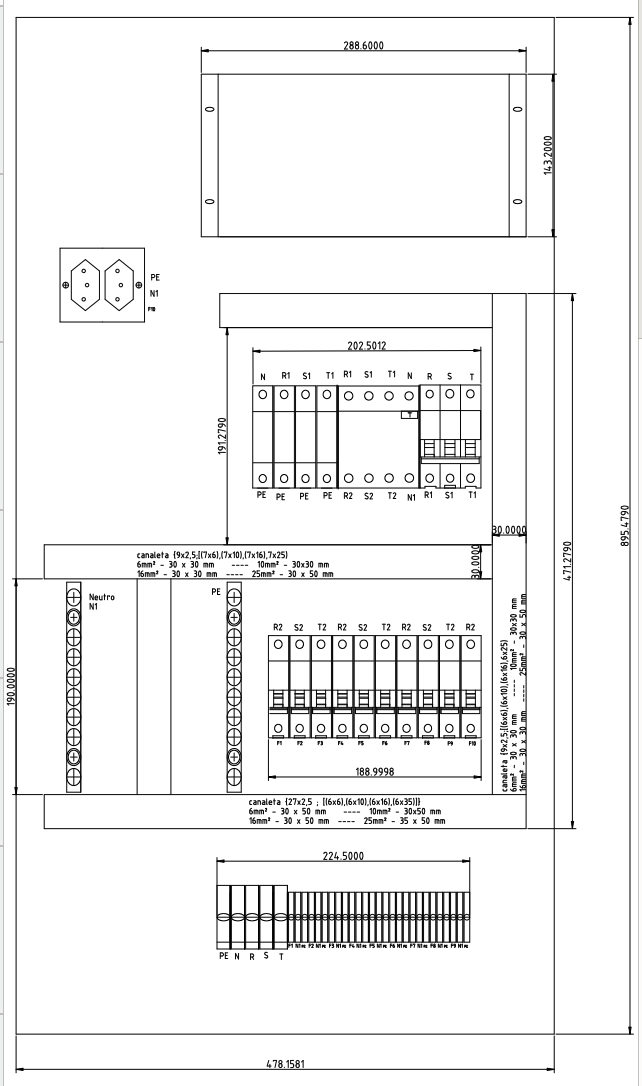
\includegraphics[width=\textwidth]{image/QD9x3tc.png}
    %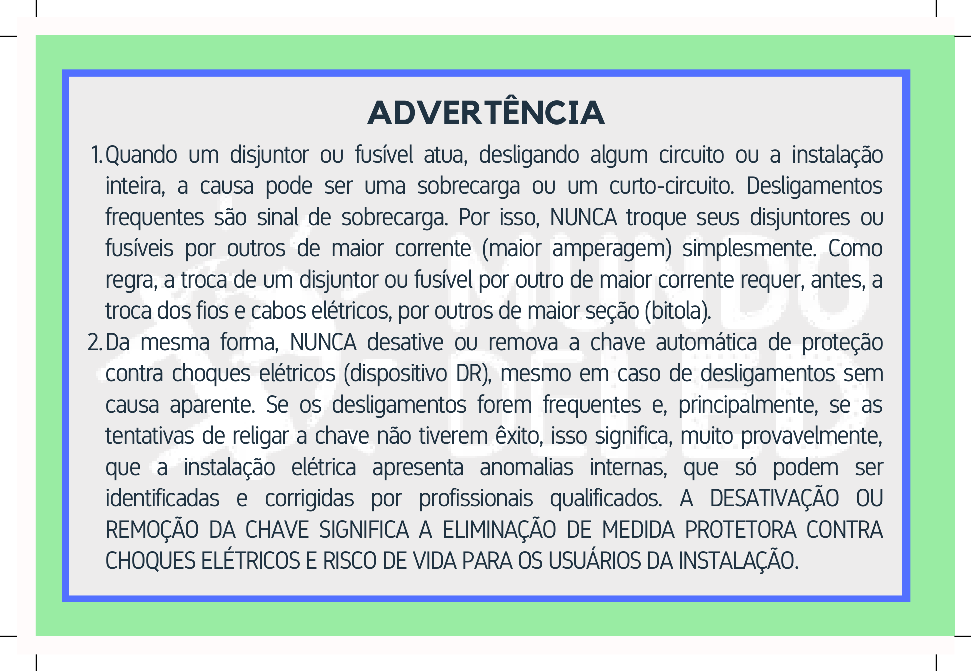
\includegraphics[width=4cm]{image/EtiqAdvQD.pdf}
    \caption{Layout em escala do Quadro Terminal 9x3T completo}
   \label{fig:QDlayout9x3}
\end{figure}
%\begin{figure}[h]
%    \centering
%    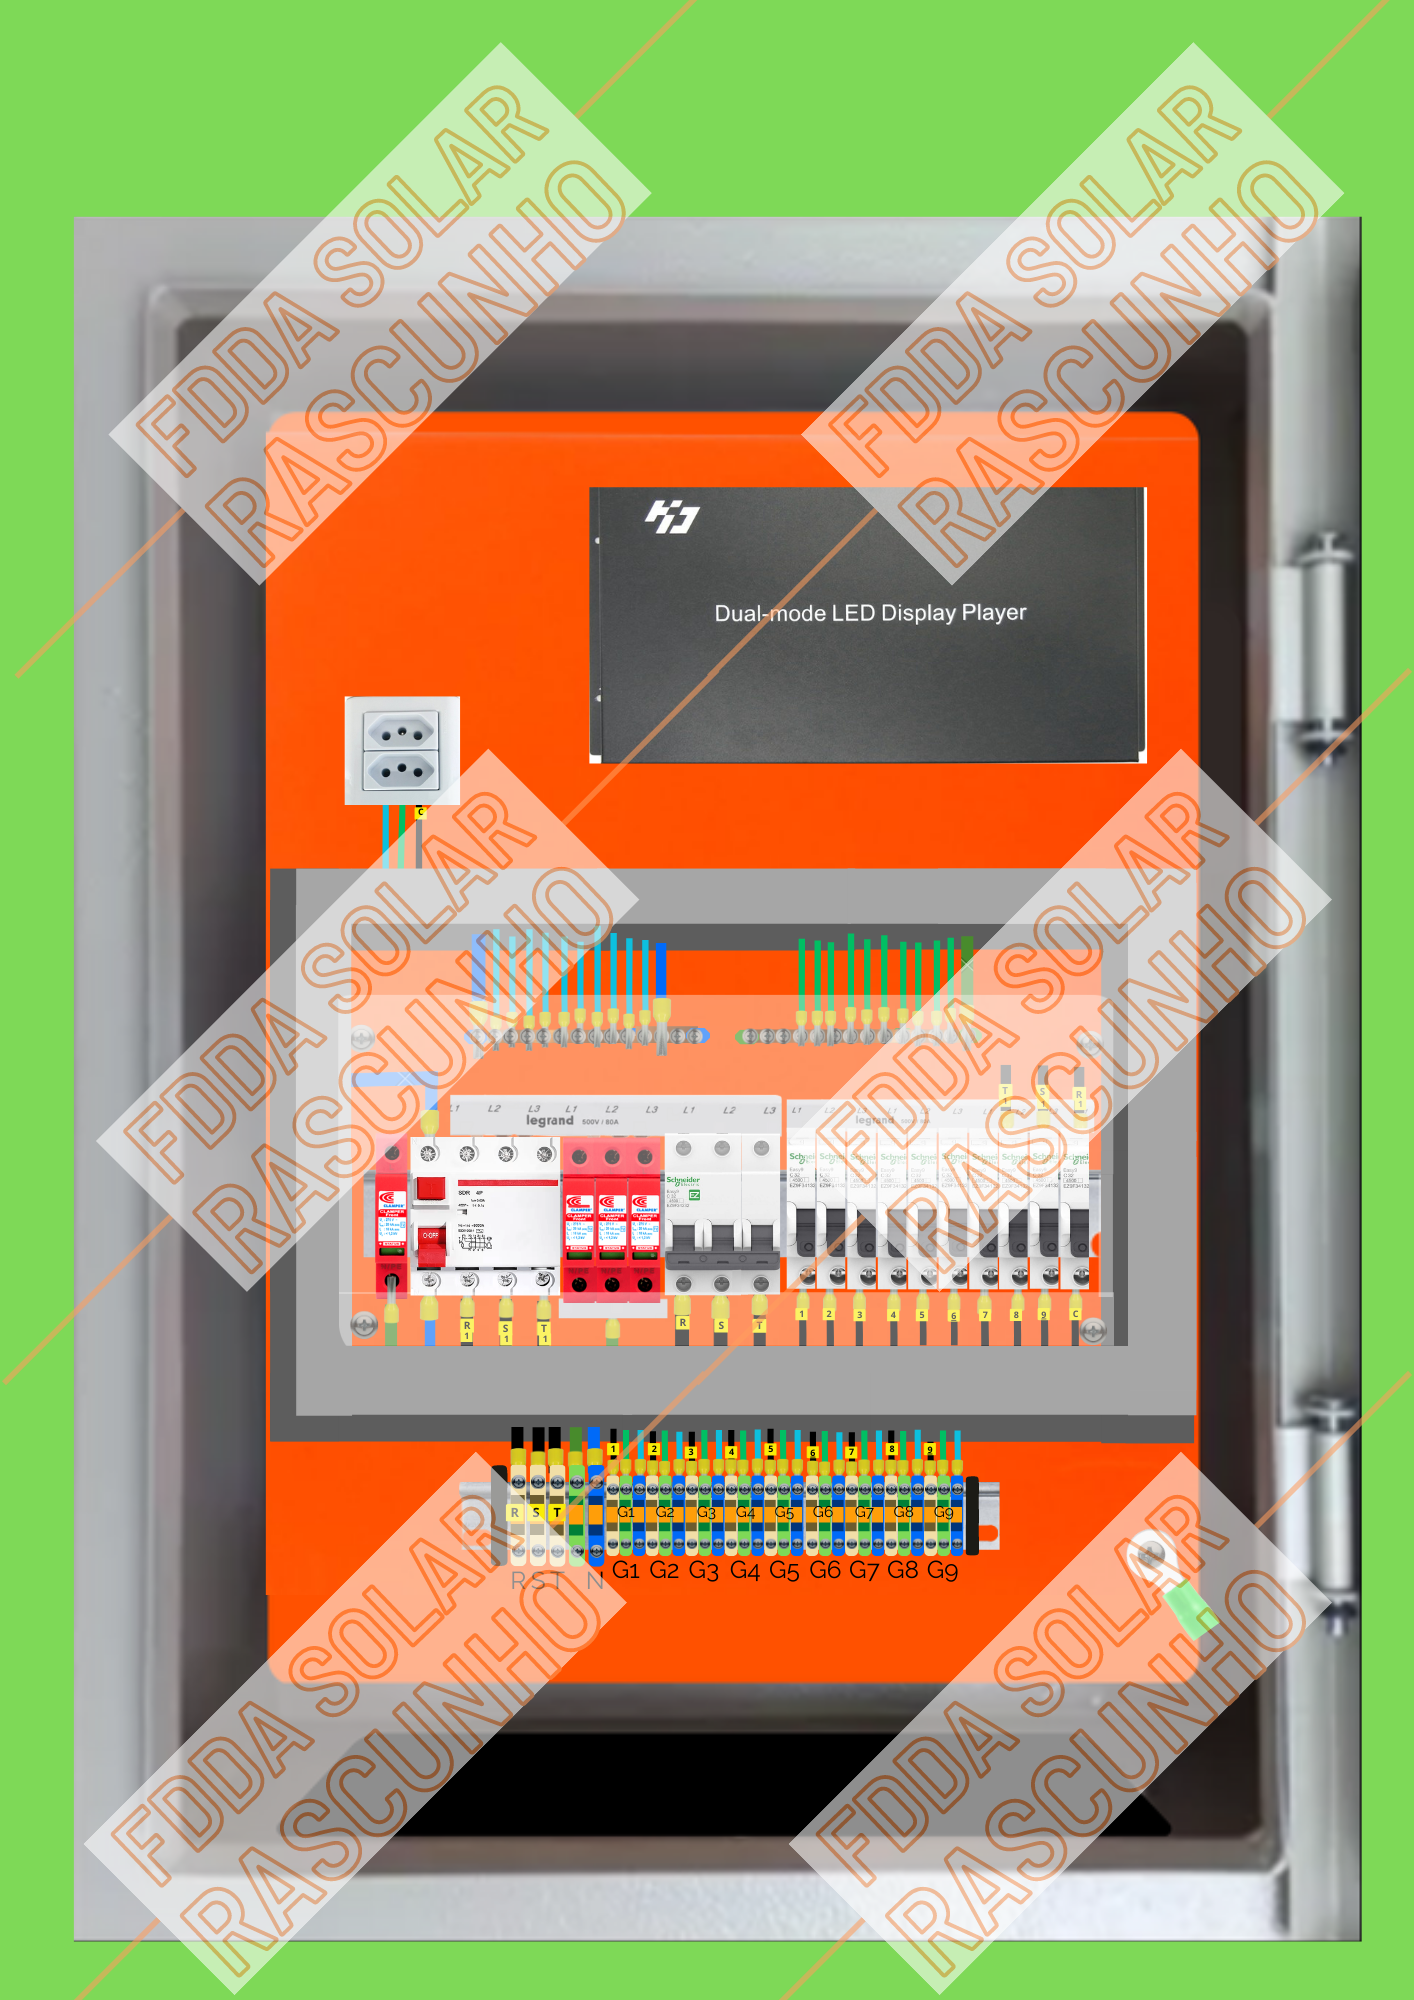
\includegraphics[width=0.4\textwidth]{image/3.png}
%    %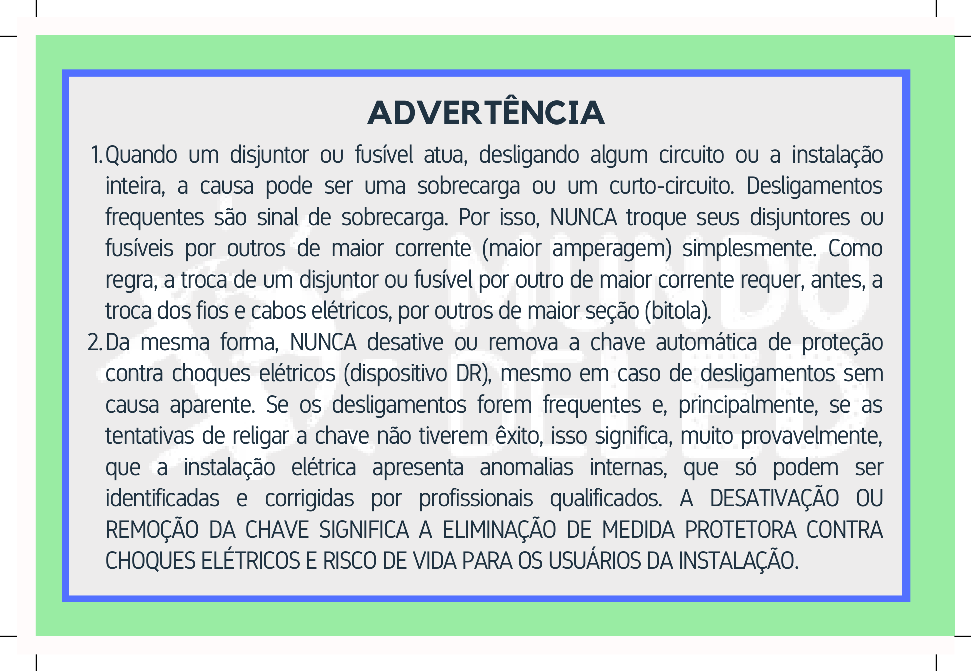
\includegraphics[width=4cm]{image/EtiqAdvQD.pdf}
%    \caption{Representação gráfica do layout interno do quadro de energia para o Painel 9x3T completo}
%   \label{fig:QDTddd}
%\end{figure}


\section{Lista de materiais}



\section{Montagem do Quadro}
\begin{itemize}
\item Qual tipo de quadro
\subitem para area externa ou interna, determina o grau de proteção dos componentes
\item Simples ou completo, determina quais componentes serão utilizados
\item ferramentas necessárias
\item  separar material necessário
\item determinar a localização dos componentes (layout)
\item fixar os componentes
\item fazer a ligação conforme projeto
\item testar
\item finalizar colocando os adesivos 
\item embalar com o manual de instalação. 

\end{itemize}

\subsection{Identificações e adesivos}
\begin{enumerate}
\item Identificar as fase com anilhas. Os fios de neutro serão identificados pela cor azul clara, e o aterramento por cabos de cor verde ou verde e amarelo padrão aterramento. Nos caso não possíveis a distinção por cores usar anilhas de identificação.
\item Colocar adesivos de identificação de entrada de energia e saída para o painel dos fios de fase, aterramento e neutro.
\item  Colocar adesivo de identificação do lado externo da porta, da porta (Figura \ref{fig:advQD_2}).
\item Fixar a Advertência na parte interna da porta do QD, como Figura \ref{fig:advQD_1}
\end{enumerate}


%\begin{figure}[ht]
%    \centering
%    %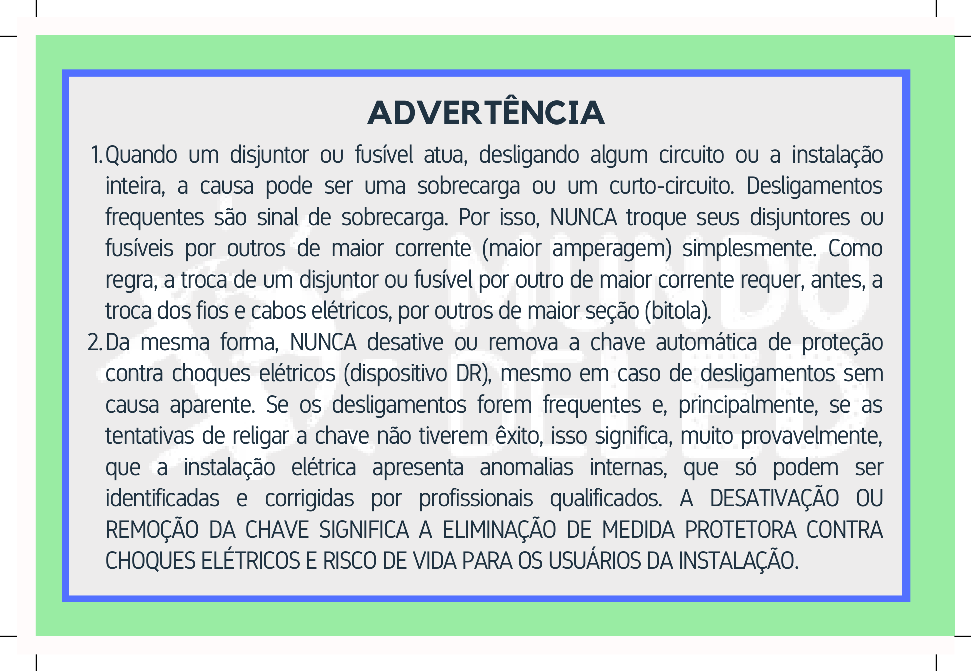
\includegraphics{image/EtiqAdvQD.pdf}
%    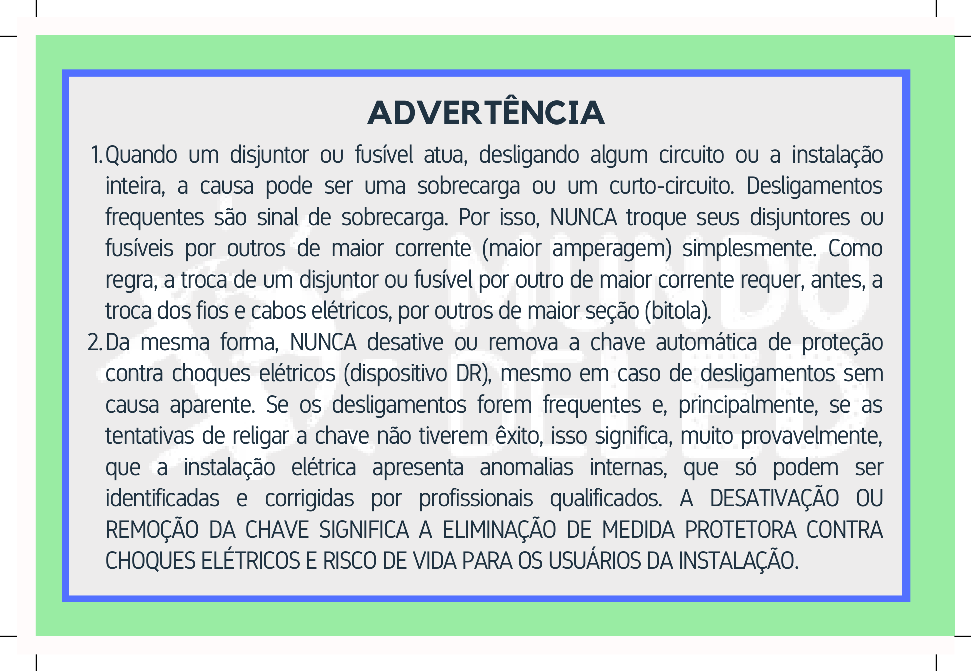
\includegraphics[width=4cm]{image/EtiqAdvQD.pdf}
%    \caption{Placa/ Adesivo de advertência para ser fixada na parte interna da porta do QD.}
   
%\end{figure}

\begin{figure}
\centering
\begin{subfigure}{0.4\textwidth}
	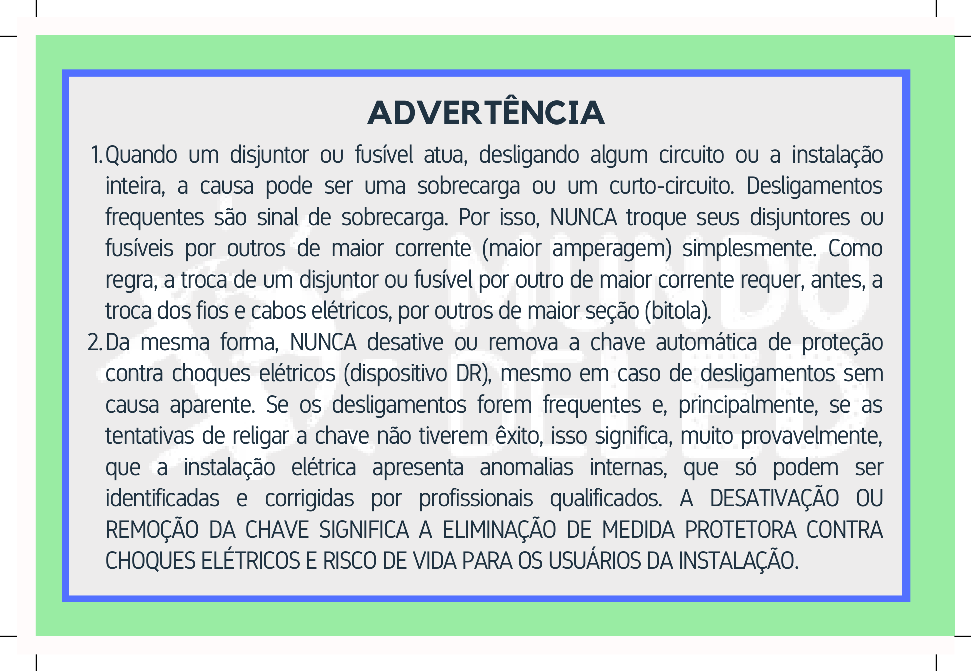
\includegraphics[width=\textwidth]{image/EtiqAdvQD.pdf}
	\caption{Advertência.}
	\label{fig:advQD_1}
\end{subfigure}
\hfill
\begin{subfigure}{0.4\textwidth}
    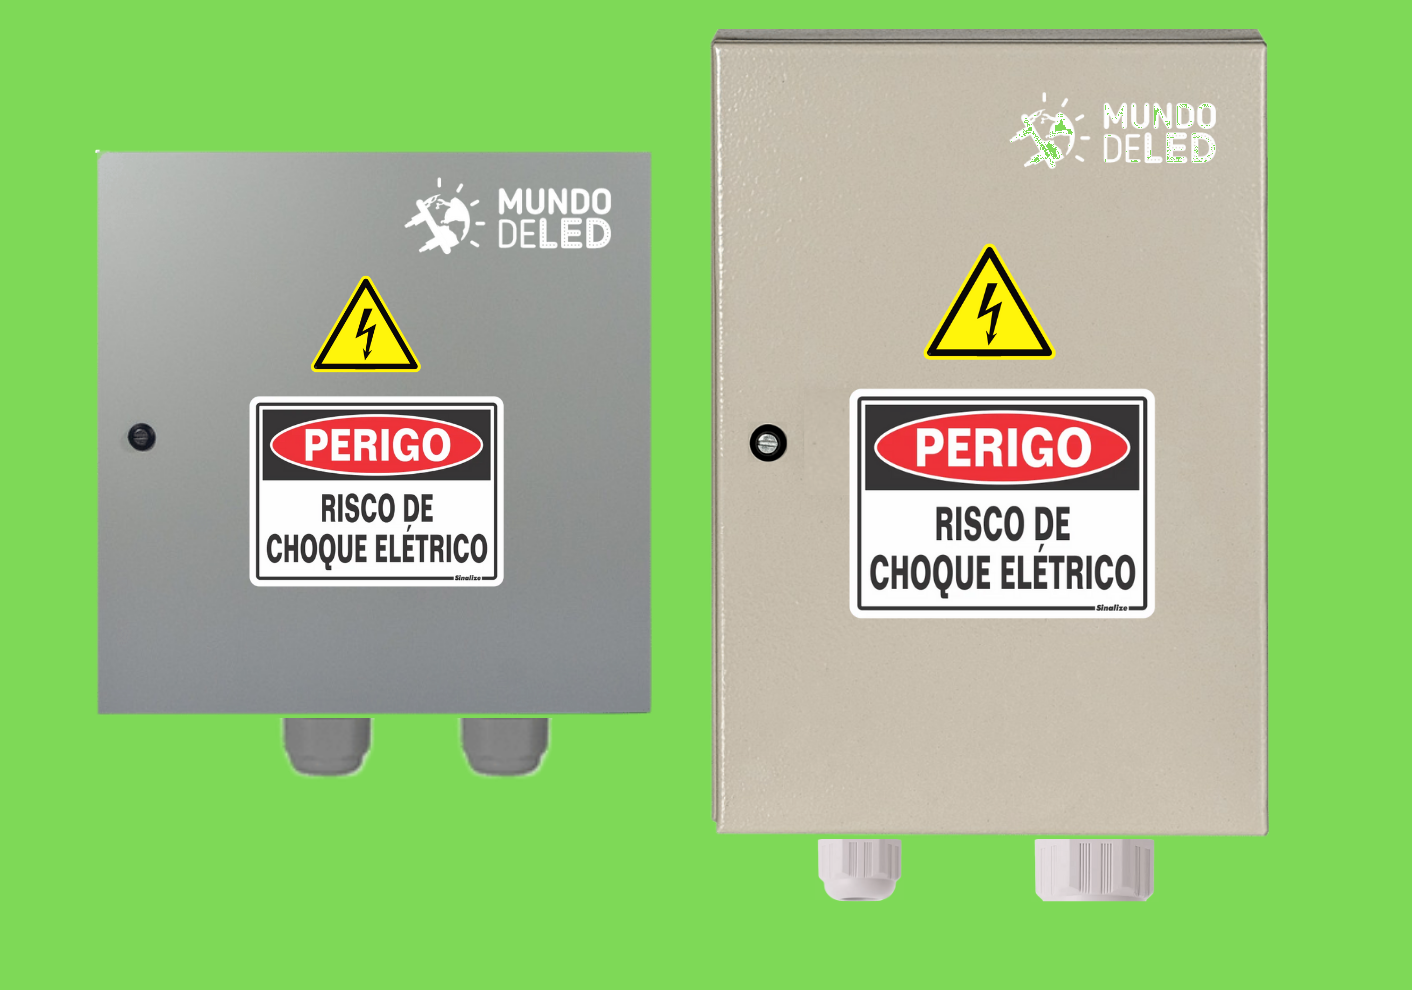
\includegraphics[width=\textwidth]{image/2.png}
    \caption{Risco de Choque}
    \label{fig:advQD_2}
\end{subfigure}
\caption{Placa/ Adesivo de advertência para ser fixada na porta do QD.}
\label{fig:advQD}
\end{figure}
